\chapter{计算机网络}
\section{TCP/IP}
如图所以显示了TCP连接的状态转换图,其中实线是客户端,虚线是服务器。
\begin{figure} 
\centering
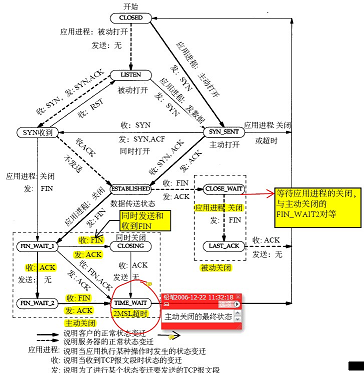
\includegraphics[width=12cm,height=10cm]{Image/TCP.png}
\caption{This is a TCP graphic}
\label{fig:tcp}
\end{figure}

\section{select/poll/epoll}
IO多路复用是指内核一旦发现进程指定的一个或者多个IO条件准备读取,它就通知该进程。IO多路复用适用如下场合:
\begin{itemize}
\item 当客户处理多个描述字时(一般是交互式输入和网络套接口),必须使用IO复用。
\item 当一个客户同时处理多个套接口时,而这种情况是可能的,但很少出现。
\item 如果一个TCP服务器既要处理监听套接口,又要处理已连接套接口,一般也要用到IO复用。
\item 如果一个服务器即要处理TCP,又要处理UDP,一般要使用IO复用。
\item 如果一个服务器要处理多个服务或多个协议,一般要使用IO复用。
\end{itemize}
与多进程和多线程技术相比,IO多路复用技术的最大优势是系统开销小,系统不必创建进程/线程,也不必维护这些进程/线程,从而大大减小了系统的开销。常见以下三种方式实现IO多路复用。
\subsection{select}
select函数原型如下:\\
int select(int maxfdp1,$fd\_set$ *readset,$fd\_set$ *writeset,$fd\_set$ *exceptset,const struct timeval *timeout) \\
返回值:就绪描述符的数目,超时返回0,出错返回-1
函数中各个参数:
\begin{itemize}
\item maxfdp1指定待测试的描述字个数,它的值是待测试的最大描述字加1。
\item 中间的三个参数readset、writeset和exceptset指定我们要让内核测试读、写和异常条件的描述字。如果对某一个的条件不感兴趣,就可以把它设为空指针。struct $fd\_set$可以理解为一个集合,这个集合中存放的是文件描述符,可通过以下四个宏进行设置:\\
void $FD\_ZERO$($fd\_set$ *fdset);           //清空集合               \\
void $FD\_SET$(int fd, $fd\_set$ *fdset);   //将一个给定的文件描述符加入集合之中 \\
void $FD\_CLR$(int fd, $fd\_set$ *fdset);   //将一个给定的文件描述符从集合中删除 \\
int $FD\_ISSET$(int fd, $fd\_set$ *fdset);   // 检查集合中指定的文件描述符是否可以读写 \\
\item timeout告知内核等待所指定描述字中的任何一个就绪可花多少时间。
这个参数有三种可能:永远等待下去、等待一段固定时间、根本不等待。
\end{itemize}
\subsection{poll}
poll的机制与select类似,与select在本质上没有多大差别,管理多个描述符也是进行轮询,根据描述符的状态进行处理,但是poll没有最大文件描述符数量的限制。poll和select同样存在一个缺点就是,包含大量文件描述符的数组被整体复制于用户态和内核的地址空间之间,而不论这些文件描述符是否就绪,它的开销随着文件描述符数量的增加而线性增大。

poll函数原型如下:\\
\centerline{int poll ( struct pollfd *fds, unsigned int nfds, int timeout);}\\
pollfd结构体定义如下:
\begin{lstlisting}[language={[ANSI]C},numbers=left,numberstyle=\tiny,%frame=shadowbox,
   rulesepcolor=\color{red!20!green!20!blue!20},
   keywordstyle=\color{blue!70!black},
   commentstyle=\color{blue!90!},
   basicstyle=\ttfamily]
struct pollfd{ 
    int fd;         /* 文件描述符 */ 
    short events;         /* 等待的事件 */ 
    short revents;       /* 实际发生了的事件 */ 
} ; 
\end{lstlisting}

每一个pollfd结构体指定了一个被监视的文件描述符,可以传递多个结构体,指示poll()监视多个文件描述符。每个结构体的events域是监视该文件描述符的事件掩码,由用户来设置这个域。revents域是文件描述符的操作结果事件掩码,内核在调用返回时设置这个域。events域中请求的任何事件都可能在revents域中返回。

成功时,poll()返回结构体中revents域不为0的文件描述符个数;如果在超时前没有任何事件发生,poll()返回0;失败时,poll()返回-1,并设置errno为下列值之一:\\
  EBADF         一个或多个结构体中指定的文件描述符无效。\\
  EFAULTfds   指针指向的地址超出进程的地址空间。\\
  EINTR      请求的事件之前产生一个信号,调用可以重新发起。\\
  EINVALnfds  参数超出PLIMIT\_NOFILE值。\\
  ENOMEM       可用内存不足,无法完成请求。\\
\subsection{epoll}
epoll支持水平触发和边缘触发,最大的特点在于边缘触发,它只告诉进程哪些fd刚刚变为就绪态,并且只会通知一次。此外epoll通过使用mmap减少复制开销。还有一个特点是,epoll使用“事件”的就绪通知方法,通过epoll\_ctl注册fd,一旦该fd就绪,内核就会采用类似callback的回调机制激活该fd,epoll\_wait便可以收到通知。

epoll的两种触发模式:LT(level trigger)和ET(edge trigger),LT模式是默认模式,两者却别有:
\begin{itemize}
\item LT模式:当epoll\_wait检测到描述符事件发生并将次事件通知应用程序,应用程序可以不立即处理该事件。下次调用epoll\_wait时,会再次相应应用程序并通知此事件。
\item ET模式:当epoll\_wait检测到描述符事件发生并将次事件通知应用程序,应用程序必须立即处理该事件。如果不处理,则下次调用epoll\_wait时,不会再次相应应用程序并通知此事件。
\end{itemize}
ET模式很大程度上减少了epoll事件被重复触发的次数,因此效率比LT高。epoll工作在ET模式的时候,必须使用非阻塞套接口,以避免由于一个文件句柄的阻塞读/阻塞写操作把处理多个文件描述符的任务饿死。\\
epoll操作的三个接口定义如下:\\
\#include <sys/epoll.h>\\
int epoll\_create(int size);\\
int epoll\_ctl(int epfd,int op,int fd,struct epoll\_event *event);\\
int epoll\_wait(int epfd,struct epoll\_event *events,int maxevents,int timeout);\\
\begin{lstlisting}[language={[ANSI]C},numbers=left,numberstyle=\tiny,%frame=shadowbox,
   rulesepcolor=\color{red!20!green!20!blue!20},
   keywordstyle=\color{blue!70!black},
   commentstyle=\color{blue!90!},
   basicstyle=\ttfamily]
struct epoll_event{ 
	__uint32_t events; /*Epoll events*/
	epoll_sata_t data; /*User data variable */
} ; 
\end{lstlisting}

\subsection{select、poll、epoll对比}
	\begin{table}[htbp]
		\caption{对比表格}
		\centering
		\begin{tabular}{cccc}
			\toprule
			&Select&Poll&Epoll\\
			\midrule
			支持最大连接数&1024(x86) or 2048(x64)&无上限&无上限 \\
			\midrule
			支持最大连接数&1024(x86) or 2048(x64)&无上限&无上限 \\
			\midrule
			支持最大连接数&1024(x86) or 2048(x64)&无上限&无上限 \\
			\bottomrule
		\end{tabular}
	\end{table}
